\section{Experimental design and evaluation}\label{ch:method}

The main experiment evaluated later MLII beats from patients whose earlier
labelled ECG was available during development. Beats were split in
chronological order within each record. This design measures performance on
known patients. The final segment had been viewed during earlier development,
so the reported results form a retrospective evaluation.

\subsection{Evaluation workflow}

Figure~\ref{fig:method-workflow} shows how accepted beats are allocated to
model selection, final refitting, and testing. The normal
autoencoder was already frozen from NSRDB. The supervised experiment then used
only MITDB MLII beats. Candidate models were selected with earlier temporal
regions, refitted before the test boundary, and evaluated only on the final
20\% of accepted beats.

\begin{figure}[H]
\centering
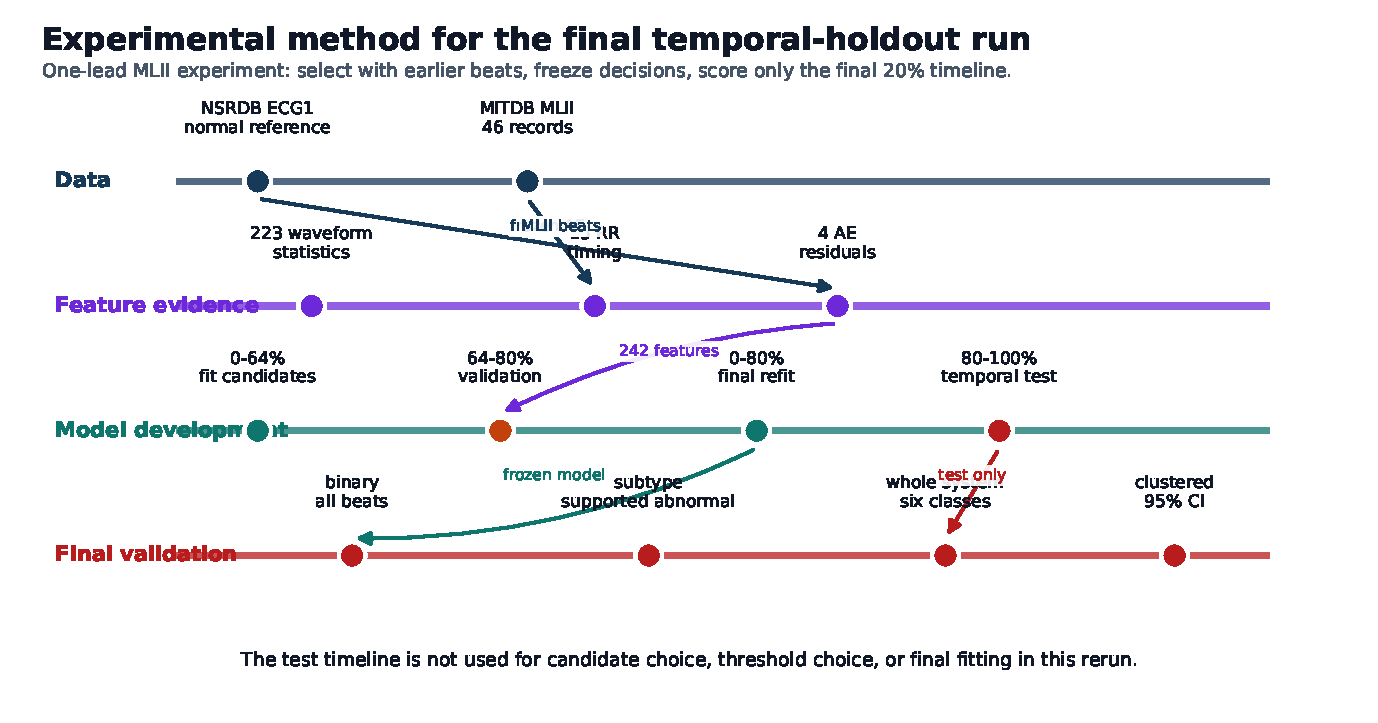
\includegraphics[width=.98\textwidth]{pic/generated/method_final_workflow.pdf}
\caption[Chronological model selection, refitting, and final testing.]{Chronological
selection, refitting, and testing by accepted-beat order. Selection excludes
16 beats before both boundaries; refitting retains only the exclusion before
the test. The test region was observed during earlier development.}
\label{fig:method-workflow}
\end{figure}

\subsection{Research objective and success conditions}

The final experiment asks:
\begin{quote}
After the model has access to the earlier ECG of each patient, how accurately
does it classify that patient's later ECG?
\end{quote}

The primary outcome is whole-system six-class accuracy on the final 20\%
temporal holdout. The planned success conditions were:
\begin{enumerate}
    \item pooled whole-system accuracy above 90\%;
    \item lower bound of the equal-subject 95\% confidence interval above
    90\%; and
    \item total confidence-interval width no greater than three percentage
    points.
\end{enumerate}
The secondary target was recall above 90\% for each supported abnormal
group. Macro F1 and per-class results were also examined because overall
accuracy can hide poor performance on a smaller class.

\subsection{Separation of normal-reference and supervised development}

The data allocation in Section~\ref{ch:data} uses 15 NSRDB subjects for
autoencoder fitting and three separate subjects for checkpoint validation.
The normal-reference checkpoint is frozen before supervised development.
NSRDB windows do not enter the final MITDB temporal test, and MITDB class
labels do not update the autoencoder. The archived NSRDB scaling is retained;
it differs from the beat-local standardisation of supervised MLII windows,
as documented in Section~\ref{sec:method-real-case}.

Both supervised models use the 242-value representation specified in
Section~\ref{ch:architecture}. The fitting equations and numerical examples
are given in Section~\ref{sec:method-training-inference}; the remainder of
this section defines how that procedure was selected and evaluated.

\subsection{Temporal split}

The eligible supervised records are the 46 MITDB records that contain MLII.
Records 102 and 104 were excluded before fitting because their available leads
are V5 and V2, not MLII. Records 201 and 202 are treated as one subject cluster
for uncertainty analysis because they belong to the same person.

Every eligible record is kept in chronological order. Percentages refer to
accepted-beat counts, not exact elapsed recording time. With $n_r$ accepted
beats, the cuts are $\lfloor0.64n_r\rfloor$ and $\lfloor0.80n_r\rfloor$:
\begin{enumerate}
    \item the first 64\% is the candidate-training region;
    \item a 16-beat gap is removed before validation during candidate
    selection;
    \item the 64--80\% region is the validation region;
    \item a 16-beat gap is removed before the final temporal test; and
    \item the final 20\% is the fixed temporal test.
\end{enumerate}
For final fitting, the selected binary and subtype models are refitted on the
earlier 80\% development region after the 16-beat boundary gap before the test
is removed. The test segment itself remains intact.

\begin{figure}[H]
\centering
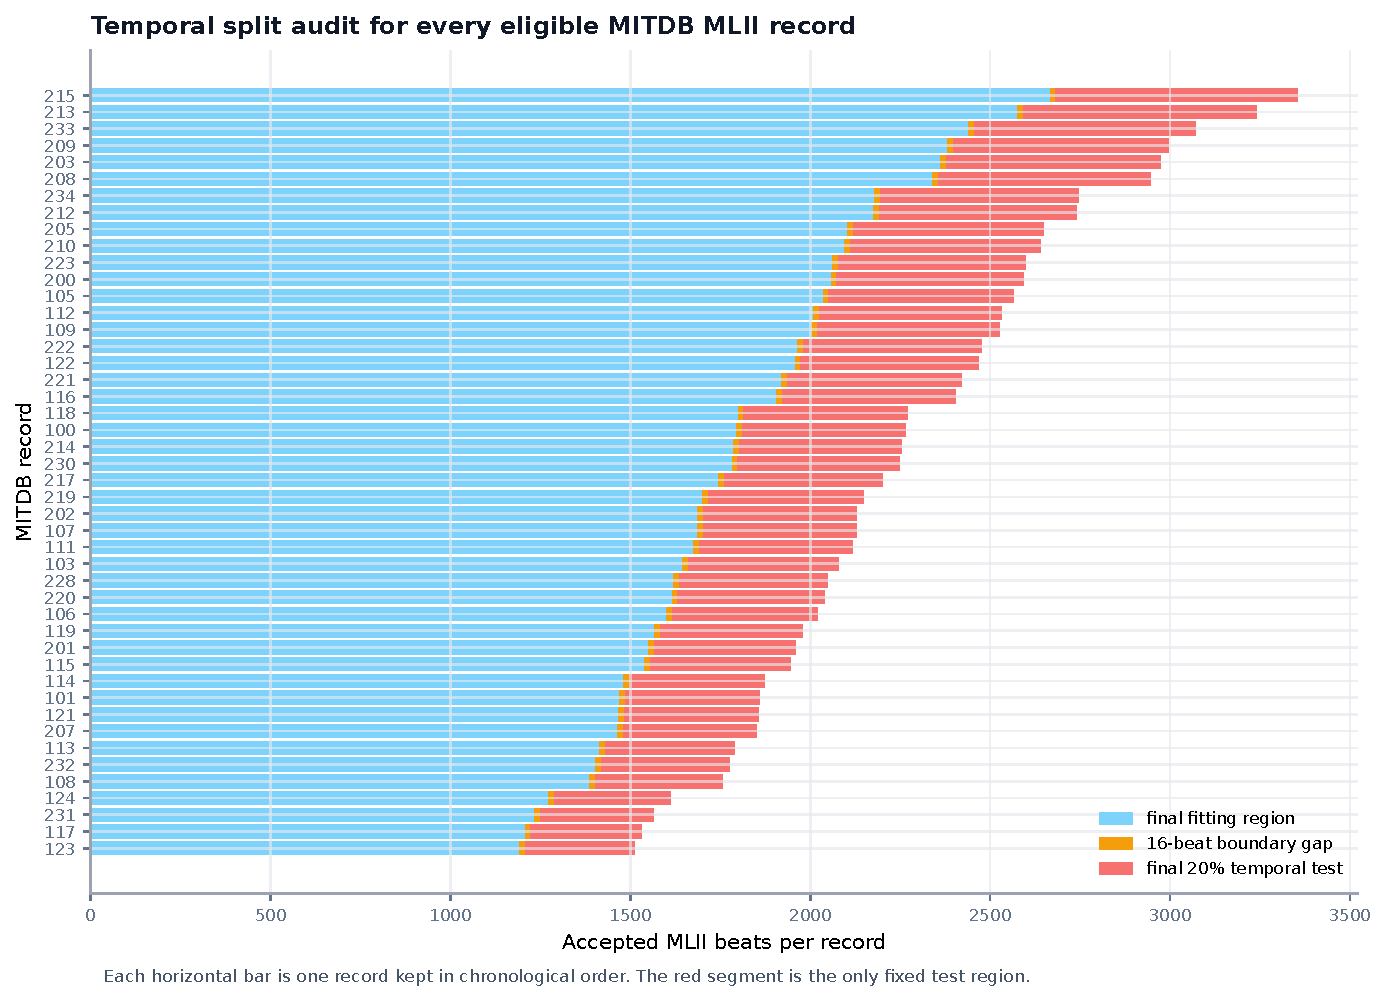
\includegraphics[width=.98\textwidth,height=.70\textheight,keepaspectratio]{pic/generated/method_temporal_split_audit.pdf}
\caption{Temporal split audit for every eligible MITDB MLII record. Blue beats
are available for final fitting, yellow beats are the boundary gap before the
test, and red beats are the held-out final 20\% temporal test.}
\label{fig:method-split-audit}
\end{figure}

The final held-out test contains 20,969 accepted beats. These are later beats
from known patients, not beats from unseen patients. The method prevents signal
overlap across the test boundary, but it intentionally keeps patient overlap.

\subsection{Model selection and final fitting}

Model selection uses only the earlier temporal validation region. In this
rerun, the final 20\% test region does not choose the candidate, threshold, or
hyperparameters.

Three binary Extra Trees candidates were fitted on the earlier candidate
region and ranked by validation balanced accuracy, then by F1. Three subtype
Extra Trees candidates were fitted only on supported abnormal candidate beats
and ranked by validation macro F1, then by accuracy. Figure~\ref{fig:method-model-selection}
shows the validation scores that selected the final pair.

The candidate-fitting rows, validation rows, sample weights, and final refit
are defined mathematically in Section~\ref{sec:method-training-inference}.
After selection, the binary model was refitted on all 83,050 eligible
development beats and the subtype model on 28,758 supported abnormal
development beats. The selected threshold was retained. Thus validation
measures model-selection performance, while the final temporal segment
measures the frozen refits under the stated retrospective protocol.

\begin{figure}[H]
\centering
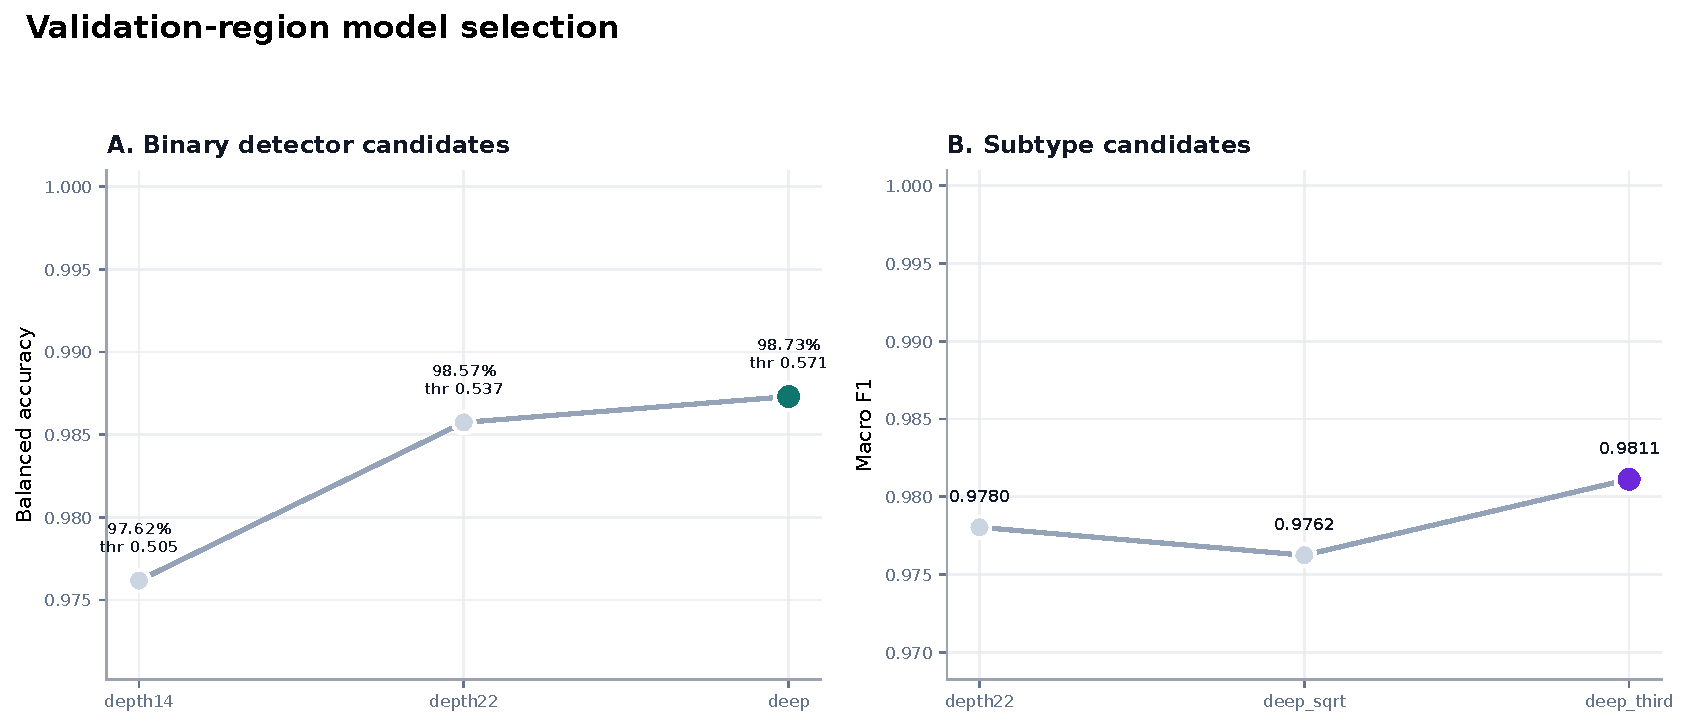
\includegraphics[width=.98\textwidth]{pic/generated/method_model_selection.pdf}
\caption{Model selection on the 64--80\% validation region. The binary detector
is selected by balanced accuracy and F1; the subtype classifier is selected by
macro F1 and accuracy.}
\label{fig:method-model-selection}
\end{figure}

The selected binary detector was the fully grown 240-tree candidate with
square-root feature sampling, minimum leaf size one, and record-weighting
power 0.35. Its validation-selected abnormal threshold was 0.5708333. The
selected subtype classifier was the fully grown 260-tree candidate with
a feature-sampling fraction of 0.33, minimum leaf size one, and record-weighting power
0.25. After selection, the binary model was refitted on all development beats,
whereas the subtype model was refitted only on supported abnormal development
beats.

\subsection{Evaluation order}

The three evaluation populations answer different questions about the
hierarchy defined in Section~\ref{ch:architecture}.

\begin{figure}[H]
\centering
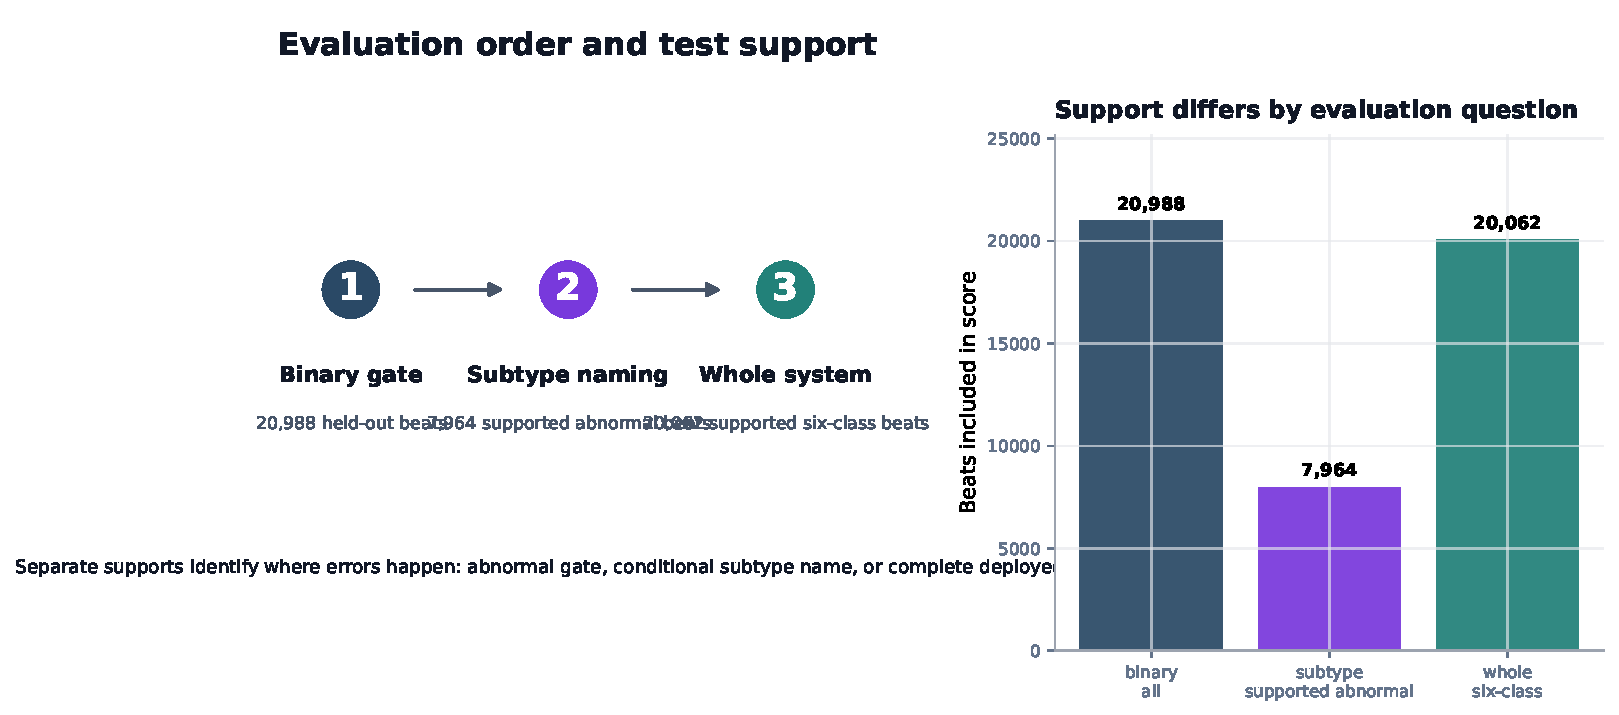
\includegraphics[width=.98\textwidth]{pic/generated/method_evaluation_order.pdf}
\caption[Populations used for the three evaluation questions.]{Populations used
for the three evaluation questions. Conditional subtype scoring uses true
supported abnormal beats independently of the gate. Complete-system scoring
uses the gate and subtype model together. The populations overlap; unsupported
abnormal labels enter only the binary evaluation.}
\label{fig:method-evaluation-order}
\end{figure}

The temporal evaluation uses three sets of beats:
\begin{enumerate}
    \item binary abnormality detection on all 20,969 held-out beats, including
    unsupported abnormal MITDB symbols;
    \item conditional subtype classification on 7,958 true supported abnormal
    beats; and
    \item whole-system N/PVC/PAC/LBBB/RBBB/AFib classification on 20,043
    supported held-out beats.
\end{enumerate}
The 926 unsupported abnormal beats are useful for testing the binary
normal/abnormal gate, but they are not scored in the six-class whole-system
confusion matrix.

\subsection{Limited external evaluation protocol}\label{sec:external-protocol}

After model fitting, the fixed hierarchy and threshold were applied to
complete INCART records I01 and I02. These were the two lead-II recordings
already cached locally at the start of the external evaluation. Selection was by local
availability, not measured performance. This is a convenience sample.
INCART contains 75 half-hour records from 32 source patients, with 12 leads
sampled at 257 Hz \cite{incartdb}. I01 and I02 both carry the header identifier
\emph{patient 1}: the two records represent one independent source patient.

Standard lead II is a practical external counterpart to MITDB MLII, not an
identical lead. This check combines source, acquisition and lead differences.
Scoring uses annotated beats, not live R-peak detections.

No external labels were used to refit the models or adjust the threshold.
The result is an exploratory transfer check; one source patient cannot
support a patient-cluster population confidence interval. Performance is
reported in Section~\ref{sec:external-incart}.

\subsection{Metrics}

For binary detection, an abnormal beat is the positive class. $TP$ and $TN$
are correctly classified abnormal and N beats; $FP$ is an N beat predicted
as abnormal, and $FN$ is an abnormal beat predicted as N. The metrics are
\begin{align}
 \mathrm{Accuracy}&=\frac{TP+TN}{TP+TN+FP+FN},\\
 \mathrm{Sensitivity}&=\frac{TP}{TP+FN},\\
 \mathrm{Specificity}&=\frac{TN}{TN+FP},\\
 \mathrm{Balanced\ accuracy}&=\frac{\mathrm{Sensitivity}+\mathrm{Specificity}}{2}.
\end{align}
For each output class $c$, the remaining classes are treated as negative
when calculating
\begin{align}
 \mathrm{Precision}_c&=\frac{TP_c}{TP_c+FP_c},\\
 \mathrm{Recall}_c&=\frac{TP_c}{TP_c+FN_c},\\
 F1_c&=\frac{2\,\mathrm{Precision}_c\mathrm{Recall}_c}
 {\mathrm{Precision}_c+\mathrm{Recall}_c}.
\end{align}
Macro F1 is the unweighted mean of class F1 values. It gives PAC the same
weight as N even though N contains many more beats. The saved scoring code
assigns zero when a precision, recall, or F1 denominator is zero. A class
with no reference examples still has no empirically estimable sensitivity;
the numerical convention does not supply evidence about that class.

Two accuracy summaries are reported. Pooled beat accuracy gives every beat
equal weight. Equal-subject accuracy first calculates accuracy within each of
the 45 eligible subject clusters and then gives every subject equal weight:
\begin{equation}
 A_{macro}=\frac{1}{45}\sum_{s=1}^{45}A_s.
 \label{eq:subject-macro}
\end{equation}
The equal-subject mean is used for uncertainty analysis so that subjects
with more beats do not receive more weight. For conditional subtype accuracy,
only subjects with supported abnormal test beats have a defined score; the
mean uses that smaller set of subjects.

\subsection{Subject-clustered confidence interval}

The primary 95\% confidence interval uses a non-parametric percentile
bootstrap:
\begin{enumerate}
    \item keep every beat from one subject together;
    \item treat records 201 and 202 as one subject cluster;
    \item sample 45 subject clusters with replacement;
    \item calculate the equal-subject mean accuracy;
    \item repeat 10,000 times using seed 20260801; and
    \item take the 2.5th and 97.5th percentiles.
\end{enumerate}
For conditional subtype accuracy, a sampled cluster without supported
abnormal test beats has an undefined score and is omitted from that
replicate's mean. The resampling still draws from all 45 clusters; the
number of defined subtype scores can therefore vary between replicates.
These intervals describe variation across the evaluated subject clusters with
the fitted model held fixed. They do not include retraining variability,
uncertainty from earlier test exposure, or a new population shift.
Resampling individual beats can create an artificially narrow interval
because adjacent beats from the same recording are correlated. The clustered
bootstrap keeps that dependence \cite{rutter2000clustered}.

\subsection{Exploratory tests against the 90\% target}

The confidence interval is the primary statistical evidence. Two
non-parametric tests provide supplementary, exploratory analyses. The exact one-sided sign
test asks whether more than half of subjects exceed 90\%. The one-sided
Wilcoxon signed-rank test asks whether subject accuracies are shifted above
90\%, under the additional symmetry assumption of a signed-rank location
test. Accuracy is bounded and has ceiling effects, so the Wilcoxon analysis is
secondary. The sign test concerns the fraction of subjects above the target,
not pooled beat accuracy. These tests are interpreted together with the confidence interval,
interval width, per-class recall, macro F1, and subject accuracy distribution.

\subsection{Reproducibility and leakage controls}

The final experiment saves the temporal boundary audit for every record, the
candidate scores, selected models, probability threshold, final confusion
matrix, per-class counts, per-subject accuracies, bootstrap seed, and headline
metrics. The rerun used seed 20260801 and did not use the final 20\% segment
for candidate selection, threshold selection, or final refitting.

The final 20\% segment had been observed during earlier system development, so
the evaluation is a retrospective rerun on previously observed data.
This prior exposure can influence design choices and cause optimism even
when the present selection code excludes test rows. It is not a confirmatory
first-use test, and the bootstrap does not correct development-selection bias. Patient overlap is
also intentional: the test is later ECG from known patients. Therefore, the
method supports a patient-adapted temporal-performance claim, not a
patient-independent generalisation claim.
